\documentclass{beamer}

\mode<presentation>
{
  \usetheme{default}
  \usecolortheme{default}
  \usefonttheme{default}
  \setbeamertemplate{navigation symbols}{}
  \setbeamertemplate{caption}[numbered]
  \setbeamertemplate{footline}[page number]
  \setbeamercolor{frametitle}{fg=white}
  \setbeamercolor{footline}{fg=black}
} 

\usepackage[english]{babel}
\usepackage[utf8x]{inputenc}
\usepackage{tikz}
\usepackage{listings}
\usepackage{courier}
\usepackage{array}
\usepackage{bold-extra}
\usepackage{minted}

\xdefinecolor{darkblue}{rgb}{0.1,0.1,0.7}
\xdefinecolor{darkgreen}{rgb}{0,0.5,0}
\xdefinecolor{darkgrey}{rgb}{0.35,0.35,0.35}
\xdefinecolor{darkorange}{rgb}{0.8,0.5,0}
\xdefinecolor{darkred}{rgb}{0.7,0,0}
\xdefinecolor{dianablue}{rgb}{0.18,0.24,0.31}
\definecolor{commentgreen}{rgb}{0,0.6,0}
\definecolor{stringmauve}{rgb}{0.58,0,0.82}

\lstset{ %
  backgroundcolor=\color{white},      % choose the background color
  basicstyle=\ttfamily\small,         % size of fonts used for the code
  breaklines=true,                    % automatic line breaking only at whitespace
  captionpos=b,                       % sets the caption-position to bottom
  commentstyle=\color{commentgreen},  % comment style
  escapeinside={\%*}{*)},             % if you want to add LaTeX within your code
  keywordstyle=\color{blue},          % keyword style
  stringstyle=\color{stringmauve},    % string literal style
  showstringspaces=false,
  showlines=true
}

\lstdefinelanguage{scala}{
  morekeywords={abstract,case,catch,class,def,%
    do,else,extends,false,final,finally,%
    for,if,implicit,import,match,mixin,%
    new,null,object,override,package,%
    private,protected,requires,return,sealed,%
    super,this,throw,trait,true,try,%
    type,val,var,while,with,yield},
  otherkeywords={=>,<-,<\%,<:,>:,\#,@},
  sensitive=true,
  morecomment=[l]{//},
  morecomment=[n]{/*}{*/},
  morestring=[b]",
  morestring=[b]',
  morestring=[b]"""
}

\title[2016-12-21-femtocode-odg]{Declarative query language for deeply nested data}
\author{Jim Pivarski}
\institute{Princeton University -- DIANA}
\date{December, 21, 2016}

\begin{document}

\logo{\pgfputat{\pgfxy(0.11, 8)}{\pgfbox[right,base]{\tikz{\filldraw[fill=dianablue, draw=none] (0 cm, 0 cm) rectangle (50 cm, 1 cm);}}}\pgfputat{\pgfxy(0.11, -0.6)}{\pgfbox[right,base]{\tikz{\filldraw[fill=dianablue, draw=none] (0 cm, 0 cm) rectangle (50 cm, 1 cm);}\tikz{\filldraw[fill=dianablue, draw=none] (0 cm, 0 cm) rectangle (4.9 cm, 1 cm);}}}}

\begin{frame}
  \titlepage
\end{frame}

\logo{\pgfputat{\pgfxy(0.11, 8)}{\pgfbox[right,base]{\tikz{\filldraw[fill=dianablue, draw=none] (0 cm, 0 cm) rectangle (50 cm, 1 cm);}}}}

% Uncomment these lines for an automatically generated outline.
%\begin{frame}{Outline}
%  \tableofcontents
%\end{frame}

%%%%%%%%%%%%%%%%%%%%%%%%%%%%%%%%%%%%%%%%%%%%%%%%%%%%%%%

\begin{frame}{I've been thinking about computational speed recently}
\vspace{0.5 cm}
\begin{itemize}\setlength{\itemsep}{0.25 cm}
\item Scientists have been thinking about single-processor efficiency for decades, and are beginning to think about scale-out.
\item Big Data community has been thinking about scale-out since its (recent) beginning, and is now thinking about single-processor efficiency.
\vspace{0.1 cm}
\begin{itemize}\setlength{\itemsep}{0.1 cm}
\item Spark's Catalyst optimizer and Project Tungsten
\item Ibis, Impala, Kudu, Dremel/Drill\ldots
\end{itemize}
\item It's not just a luxury: the time between query and the response limits a human's ability to develop instinct and see larger relationships.

\vspace{0.5 cm}
\textcolor{gray}{``Answers can change the question line\ldots\ every time.''}

\mbox{ } \hfill \textcolor{gray}{--- Adam Ant}
\end{itemize}
\end{frame}

\begin{frame}{Hurdle theory}
\vspace{0.5 cm}
\textcolor{darkblue}{My favorite metaphor for computational speed:} fast software is not like a fast runner, who has some superior intrinsic ability. All programs run at the same rate, the clock rate. But some have more hurdles on the track than others.

\vspace{0.25 cm}
\begin{center}
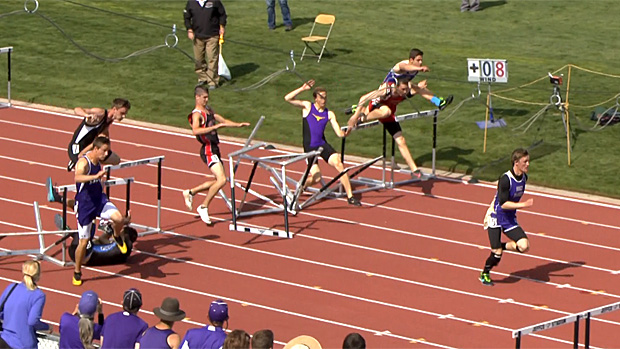
\includegraphics[width=0.7\linewidth]{hurdle9.jpg}
\end{center}
\end{frame}

\begin{frame}{But it's more than that\ldots}
\vspace{0.5 cm}
\begin{columns}
\column{0.4\linewidth}
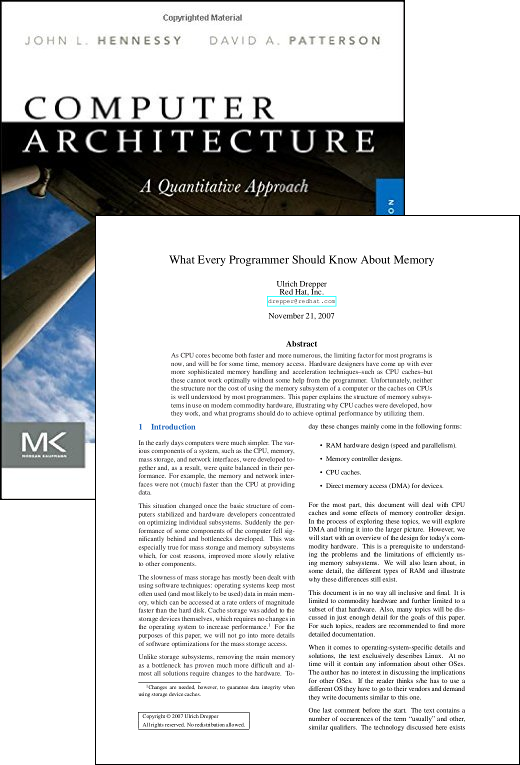
\includegraphics[width=\linewidth]{books.png}

\column{0.55\linewidth}
\textcolor{darkblue}{Gotcha:} many of these hurdles are invisible!

\vspace{0.5 cm}
Since the 1990's, improvements in processor speed have outpaced improvements in memory bandwidth, so now memory is the bottleneck.

\vspace{0.5 cm}
Also, slow operations are pipelined to optimize throughput: many clock ticks from start to finish, but a full pipeline can push through one operation per clock tick.

\vspace{0.5 cm}
``Bubbles'' in the pipe thwart this.
\end{columns}
\end{frame}

\begin{frame}[fragile]{Fast code looks like this}
\begin{center}
\begin{minipage}{0.7\linewidth}
\begin{minted}[frame=single]{c++}
for (int i = 0;  i < size;  i++)
  out[i] = in1[i] / in2[i];
\end{minted}
\end{minipage}
\end{center}

\begin{itemize}
\item Simple loop structure that the compiler can unfold.
\item Forward stride that the CPU can detect and prefetch memory. (Arrays are contiguous in memory: bonus points for proper memory-alignment.)
\item Bubble-free pipeline (except at start and end; edge effects).
\item Would allow SIMD parallelism that could be vectorized (1024 at a time in a GPU, 4 or 8 for MMX, 256 for KNL\ldots).
\end{itemize}
\end{frame}

\begin{frame}{Field is ripe with low-hanging fruit}
\vspace{0.5 cm}
\textcolor{darkblue}{I've estimated that our weeks-long physics jobs, which touch hundreds of terabytes, could be reduced to minutes or seconds.}
\begin{itemize}
\item Only need to touch $\sim$80~GB of {\it columnar} data in typical 100 million event example.
\item {\it Single} processor can load 80~GB data arrays in 20 minutes \\ (so divide by $N$, number of processors).
\item Optimized C code can perform one simple operation in 12 seconds. (Divide by $N$.)
\item Low-end GPU can perform the same operation in 5 seconds. (Divide by $N$.)
\end{itemize}

\vspace{0.5 cm}
\small
\textcolor{gray}{Actually a change in behavior: ``weeks'' are spent making private skims to perform these operations quickly offline. But a shared server with sufficient caching would allow users to calculate one plot at a time, reducing the amount of data that needs to be read/copied.}
\end{frame}






%% \begin{frame}{Two ways to more incisive data analysis}
%% \begin{columns}[t]
%% \column{0.5\linewidth}
%% \textcolor{darkblue}{\underline{Rapid, interactive queries}}

%% \vspace{0.2 cm}
%% Speed is not a luxury: the time between question and response limits a human's ability to understand and act on it.

%% \vspace{0.2 cm}
%% The reason you asked the question is still in mind.

%% \vspace{0.2 cm}
%% \begin{uncoverenv}<2->
%% \begin{itemize}
%% \item Ibis, Impala, Kudu, Drill\ldots
%% \item Usually SQL-like language
%% \item SparkSQL DataFrames
%% \end{itemize}
%% \end{uncoverenv}

%% \column{0.5\linewidth}
%% \textcolor{darkblue}{\underline{Deep manipulation}}

%% \vspace{0.2 cm}
%% Not all datasets are flat tables, especially ``data lakes'' shared for multiple purposes.

%% \vspace{0.2 cm}
%% Restructuring opens the door to finding new purposes for old data.

%% \vspace{0.2 cm}
%% \begin{uncoverenv}<2->
%% \begin{itemize}
%% \item Hadoop, PFA, custom code
%% \item ``Deployed analytic''
%% \item Spark RDDs and Datasets
%% \end{itemize}
%% \end{uncoverenv}
%% \end{columns}



%% \end{frame}




\end{document}
